\documentclass[10pt,journal]{IEEEtran}
\IEEEoverridecommandlockouts
\usepackage[spanish,es-tabla]{babel}
\renewcommand{\baselinestretch}{1.5}     %interlineado
\usepackage[utf8]{inputenc} 
\usepackage[square,numbers]{natbib}
\bibliographystyle{abbrvnat}
\usepackage{float}                      % para usar [H]
\usepackage[table,xcdraw]{xcolor}
\usepackage{amsmath,amssymb,amsfonts}
\usepackage{graphicx}
\usepackage{textcomp}
\usepackage{xcolor}

\def\BibTeX{{\rm B\kern-.05em{\sc i\kern-.025em b}\kern-.08em
    T\kern-.1667em\lower.7ex\hbox{E}\kern-.125emX}}

%---------------------------------------------------
\begin{document}

\title{Ideas de Investigación en Informática o en Ciencias de la Computación\\}
%--------------------------------------------
\author{\IEEEauthorblockN{Ciara Mendez Cruz}
\IEEEauthorblockA{\textit{} \\
\textit{Universidad Nacional de Trujillo} \\ 
\textit{Trujillo, Perú} \\
t022700920@unitru.edu.pe}}
\maketitle
%-------------------------------------------
\begin{abstract}
La informática es el proceso de resolver problemas organizacionales complejos utilizando soluciones técnicas. La razón por la que este es un campo tan importante es que las computadoras y la tecnología se han integrado en prácticamente todos los sectores económicos, industrias e incluso organizaciones que operan en la economía moderna. Por ello, es necesario continuar y practicar la investigación en este campo. Una idea de investigación que se desarrollo en el área de Internet de las cosas(Iot), fue que se diseñó, optimizó, fabricó y caracterizó un recolector de energía para aplicaciones de IoT y recolección de energía que simplemente recicla energía de radiofrecuencia (RF) a 2,4 GHz, de dispositivos Wi-Fi/WLAN cercanos y los convierte en energía de CC útil, por otro lado, en el área de Computación en la nube(Cloud Computing)  se define a la criptografía de curva elíptica (ECC) como una técnica de cifrado de clave pública basada en la teoría de la curva elíptica que se puede utilizar para crear claves criptográficas más rápidas, más pequeñas y más eficientes, la que proporcionó soluciones para un entorno seguro en la nube con un rendimiento mejorado en el uso de recursos de energía y batería de cómputo, asimismo se explican tres investigaciones más en tres áreas diferentes de las antes mencionadas en ciencias de la computación.
\end{abstract}

\begin{IEEEkeywords}
ideas, investigación, informática.
\end{IEEEkeywords}

\section{\textbf{Introducción}}
La informática es uno de los campos más amplios que existe y es la tarea más difícil encontrar el tema de investigación del cual queremos indagar dentro del campo de la informática. Con el tiempo, las innovaciones nuevas y emergentes están ocurriendo en este campo a diario. Estas innovaciones son muy útiles para la vida humana y facilitan la realización de algunas tareas. 

Por ello, en este informe se presenta información respecto a cinco ideas de investigación en informática o en ciencias de la computación para continuar con su profundización o generar ideas nuevas relacionadas a ellas. Se ha considerado para cada una de las siguientes cinco áreas de Ciencias de la Computación: Internet de las cosas (IoT), Computación en la nube (Cloud Computing), Procesamiento del lenguajes natural (PNL-Language Processing), Aprendizaje automático(ML-Machine Learning) e Inteligencia Artificial (AI-Artificial Intelligence) una investigación, el impacto que genera en la sociedad y especialmente en que consiste cada una de ellas.
%------------------------------------------
\section{\textbf{Ideas de Investigación}}
\subsection{\textbf{Internet de las cosas (IoT)}}
La comunicación de persona a persona y de persona a máquina empleada tradicionalmente ha sido reemplazada recientemente por una nueva tendencia conocida como Internet de las cosas (IoT).\par IoT permite la comunicación de dispositivo a dispositivo sin intervención humana, por lo tanto, ofrece muchos desafíos. En este paradigma, la autosostenibilidad de las máquinas debido a las capacidades energéticas limitadas presenta un gran desafío.\par
En la investigación titulada \textit{Recolección de energía usando una Rectenna de bajo costo para aplicaciones de Internet de las cosas (IoT)} \citep{internet} se diseñó, optimizó, fabricó y caracterizó un recolector de energía para aplicaciones de IoT y recolección de energía que simplemente recicla energía de radiofrecuencia (RF) a 2,4 GHz, de dispositivos Wi-Fi/WLAN cercanos y los convierte en energía de CC útil.\par
El modelo físico consta de antena, filtros, rectificador, etc. Una antena de parche rectangular está diseñada y optimizada para resonar a 2,4 GHz usando el conocido modelo de línea de transmisión, mientras que los filtros de paso de banda y de paso bajo están diseñados usando componentes agrupados. El diodo Schottky (HSMS-2820) se utiliza para la rectificación. El circuito está diseñado y fabricado utilizando el sustrato FR4 de bajo costo (h = 16 mm y r = 4.6) con dimensiones de fabricación de 285 mm × 90 mm. Se emplean periféricos de radio de software Universal y GNU Radio para medir la potencia de RF recibida, mientras que se realizan mediciones similares utilizando el analizador de espectro RyS para la validación. La potencia medida recibida es de -64,4 dBm en el puerto de salida del circuito de la rectenna. Por lo tanto, su diseño permite una implementación generalizada de dispositivos IoT de próxima generación autooperables.

\begin{figure}[H]
 \begin{center}
       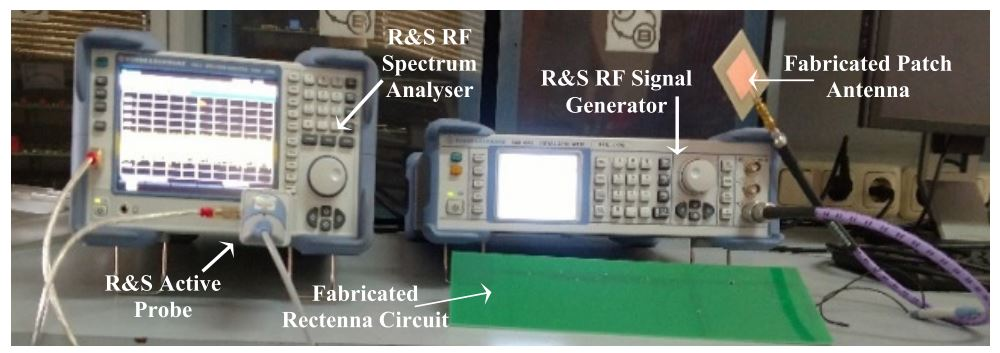
\includegraphics[width=8.5cm, height=5cm]{figuras/1.JPG}
      \caption{Montaje de medida de potencia del circuito de rectena a diferentes distancias.}
      \label{f1} 
      \end{center}
\end{figure}

\subsection{\textbf{Computación en la nube (Cloud Computing)}}
Las aplicaciones informáticas y los datos están creciendo tan rápidamente que se necesitan servidores y centros de datos cada vez más grandes para un procesamiento rápido en el tiempo requerido. Un cambio fundamental en la forma en que se entregan y compran los servicios informáticos y de tecnología de la información (TI) da como resultado el desarrollo de la computación en la nube. \par Sin embargo, la computación en la nube requiere que las organizaciones confíen en que las plataformas de un proveedor de servicios estén protegidas y brinden un nivel suficiente de integridad para los datos del cliente.\par
En la investigación titulada \textit{Criptografía de curva elíptica para proteger las aplicaciones de computación en la nube} \citep{eliptic} se define a la criptografía de curva elíptica (ECC) como una técnica de cifrado de clave pública basada en la teoría de la curva elíptica que se puede utilizar para crear claves criptográficas más rápidas, más pequeñas y más eficientes. Un factor importante es la fortaleza de la clave, es decir, la dificultad para romper la clave y recuperar el texto sin formato.\par En la investigación propusieron el esquema de criptografía de curva elíptica como una herramienta segura para modelar una plataforma segura para la aplicación en la nube.
Asimismo, se determinó que proporciona soluciones para un entorno seguro en la nube con un rendimiento mejorado en el uso de recursos de energía y batería de cómputo. Esto lo hace atractivo para aplicaciones móviles. ECC había proporcionado un modelo sólido y seguro para el desarrollo y la implementación de aplicaciones seguras en la nube. La investigación promovería la confianza en la inversión en la nube en organizaciones de pequeña y gran escala.

\begin{figure}[H]
 \begin{center}
       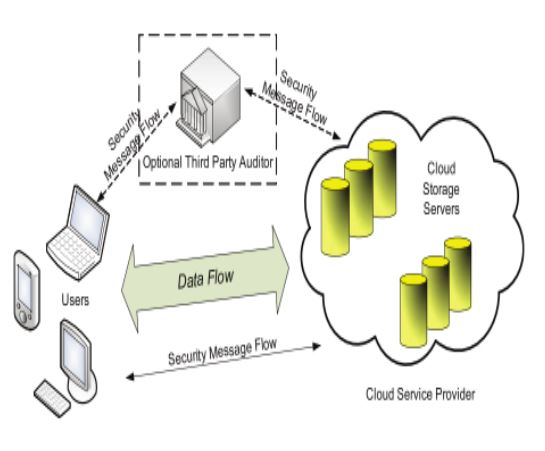
\includegraphics[width=8.5cm, height=5cm]{figuras/2.JPG}
      \caption{Arquitectura de almacenamiento de datos en la nube.}
      \label{f2} 
      \end{center}
\end{figure}

\subsection{\textbf{Procesamiento del lenguaje natural (PNL-Natural Language Processing)}}
La migración de los informes de imágenes a los sistemas de registros médicos electrónicos tiene un gran potencial en términos de avanzar en la investigación y la práctica de la radiología al aprovechar el gran volumen de datos que se actualizan, integran y comparten continuamente. Sin embargo, también existen desafíos importantes, en gran parte debido a la heterogeneidad de cómo se formatean estos datos.\par  De hecho, aunque hay un movimiento hacia informes estructurados en radiología (es decir, informes detallados jerárquicamente con el uso de terminología estandarizada), la mayoría de los informes de radiología siguen sin estructurar y utilizan un lenguaje de formato libre.\par La extracción manual de información es una tarea que requiere mucho tiempo y, a menudo, es inmanejable.\par
En la investigación titulada \textit{Tecnologías de procesamiento del lenguaje natural en investigación radiológica y aplicaciones clínicas} \citep{natural} nos explica que, los motores de búsqueda inteligentes se basan en el procesamiento del lenguaje natural (NLP), un enfoque basado en computadora para analizar texto o voz de forma libre y se pueden usar para automatizar la tarea de extracción de datos. \par Además, el objetivo general de la PNL es traducir el lenguaje humano natural a un formato estructurado (es decir, una colección fija de elementos), cada uno con un conjunto estandarizado de opciones para su valor, que los programas informáticos pueden manipular fácilmente para (entre otras cosas) ordenar en subcategorías o consulta por la presencia o ausencia de un hallazgo. Los autores de esta investigación revisan los fundamentos de la PNL y describen varias técnicas que constituyen la PNL en radiología, junto con algunas aplicaciones clave.

\subsection{\textbf{Aprendizaje automático (ML-Machine Learning)}}
La agricultura juega un papel vital en el crecimiento económico de cualquier país. Con el aumento de la población, los cambios frecuentes en las condiciones climáticas y los recursos limitados, se convierte en una tarea desafiante satisfacer los requerimientos alimentarios de la población actual. La agricultura de precisión, también conocida como agricultura inteligente, ha surgido como una herramienta innovadora para abordar los desafíos actuales en la sostenibilidad agrícola.\par
En la investigación titulada \textit{Aplicaciones de aprendizaje automático(ML) para la agricultura de precisión: una revisión exhaustiva} \citep{machine}, los autores presentan una revisión sistemática de las aplicaciones de ML en el campo de la agricultura. Las áreas que se enfocan son la predicción de parámetros del suelo como el contenido de húmedad y carbono orgánico, la predicción del rendimiento de los cultivos, la detección de enfermedades y malezas en los cultivos y la detección de especies. ML con visión por computadora se revisan para la clasificación de un conjunto diferente de imágenes de cultivo para monitorear la calidad del cultivo y la evaluación del rendimiento
\par Este enfoque se puede integrar para mejorar la producción ganadera mediante la predicción de patrones de fertilidad, el diagnóstico de trastornos alimentarios, el comportamiento del ganado basado en modelos ML utilizando datos recopilados por sensores de collar, etc. También se revisa el riego inteligente que incluye riego por goteo y técnicas de cosecha inteligentes que reducen el trabajo humano. en gran parte. \par Esta investigación demuestra cómo la agricultura basada en el conocimiento puede mejorar la productividad sostenible y la calidad del producto. predicción de rendimiento de cultivos, detección de enfermedades y malezas en cultivos y detección de especies.

\begin{figure}[H]
 \begin{center}
       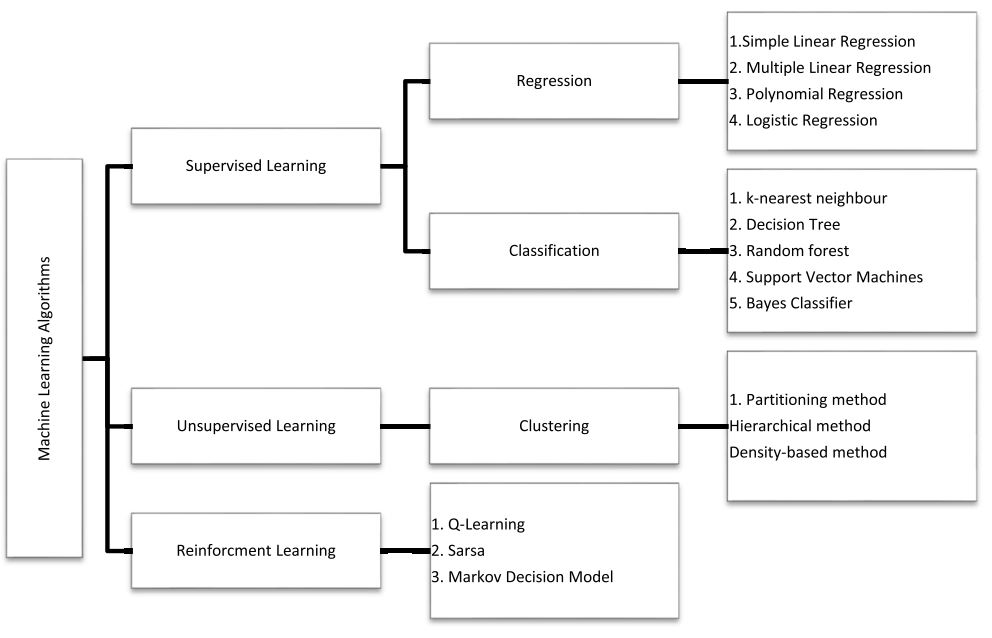
\includegraphics[width=8.5cm, height=3cm]{figuras/3.JPG}
      \caption{Categorización de algoritmos de aprendizaje automático.(ML)}
      \label{f3} 
      \end{center}
\end{figure}

\subsection{\textbf{Inteligencia Artificial(AI-Artificial Intelligence)}}
Los procesos de gestión de residuos suelen implicar numerosos parámetros técnicos, climáticos, medioambientales, demográficos, socioeconómicos y legislativos. Tales procesos no lineales complejos son difíciles de modelar, predecir y optimizar utilizando métodos convencionales.
En la investigación titulada \textit{Aplicaciones de la inteligencia artificial en la gestión de residuos sólidos: una revisión sistemática de la investigación} \citep{artificial} muestra que, recientemente, las técnicas de inteligencia artificial (IA) han cobrado impulso al ofrecer enfoques computacionales alternativos para resolver problemas de gestión de residuos sólidos (SWM). \par La IA ha sido eficiente para abordar problemas mal definidos, aprender de la experiencia y manejar la incertidumbre y los datos incompletos. Aunque se llevó a cabo una investigación significativa en este dominio, muy pocos estudios de revisión han evaluado el potencial de la IA para resolver los diversos problemas de SWM. \par En esta investigación se realizó la revisión sistemática de la literatura que compiló 85 estudios de investigación, publicados entre 2004 y 2019, analizó la aplicación de IA en varios campos de SWM, incluida la previsión de las características de los desechos, la detección del nivel del contenedor de desechos, la predicción de los parámetros del proceso, el enrutamiento de vehículos y la planificación de SWM. Esa revisión proporciona un análisis exhaustivo de los diferentes modelos y técnicas de IA aplicados en SWM, los dominios de aplicación y los parámetros de rendimiento informados, así como las plataformas de software utilizadas para implementar dichos modelos.

\begin{figure}[H]
 \begin{center}
       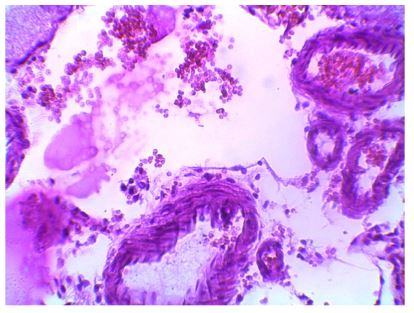
\includegraphics[width=8cm, height=2cm]{figuras/4.JPG}
      \caption{Análisis exhaustivo de los diferentes modelos y técnicas de IA aplicados en SWM.}
      \label{f4} 
      \end{center}
\end{figure}

\section{\textbf{Conclusiones}}
Este informe presentó información relevante respecto a cinco ideas de investigación en informática o en ciencias de la computación. Se ha explicado para cada una de las siguientes cinco áreas consideradas de Ciencias de la Computación: Internet de las cosas (IoT), Computación en la nube (Cloud Computing), Procesamiento del lenguajes natural (PNL-Language Processing), Aprendizaje automático(ML-Machine Learning) e Inteligencia Artificial (AI-Artificial Intelligence) una investigación, además de permitir reafirmar que la informática es un campo futurista avanzado y emergente de innovaciones importantes relacionadas con la forma de vida moderna. 
%-------------------------------------------------------
\medskip
\bibliography{refer}
\end{document}
